\clearpage
\begin{center}
\begin{longtable}{| m{4.5cm} | m{5cm} | m{4.5cm} |}\caption{Calculated equilibrium geometries for all species.}
\label{tab:pic}
\endfirsthead
\endhead
\hline
compound & Top View & Side View \\ \hline\ 
NH$_{3}$ at top active site&\makecell{  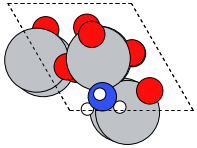
\includegraphics[width=0.30\textwidth, height=38mm]{surface_pathway/NH3-top.png}}&\makecell{  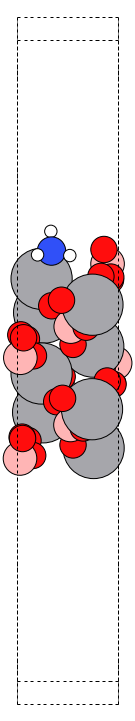
\includegraphics[width=0.15\textwidth, height=85mm]{surface_pathway/NH3-xside.png}} \\ \hline\ 
NH$_{2}$ at top active site&\makecell{  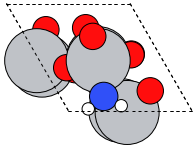
\includegraphics[width=0.30\textwidth, height=38mm]{surface_pathway/NH2-top.png}}&\makecell{  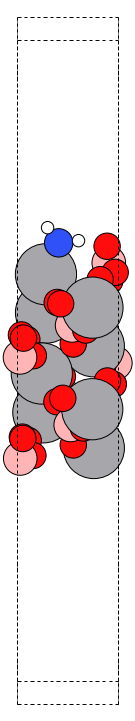
\includegraphics[width=0.15\textwidth, height=85mm]{surface_pathway/NH2-xside.png}} \\ \hline\ 
N$_{2}$H at top active site&\makecell{  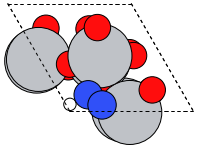
\includegraphics[width=0.30\textwidth, height=38mm]{surface_pathway/N2H-top.png}}&\makecell{  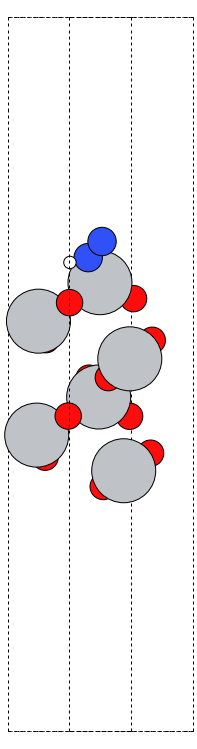
\includegraphics[width=0.15\textwidth, height=85mm]{surface_pathway/N2H-xside.png}} \\ \hline\ 
N$_{2}$H$_{2}$ at top active site&\makecell{  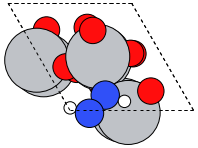
\includegraphics[width=0.30\textwidth, height=38mm]{surface_pathway/N2H2-top.png}}&\makecell{  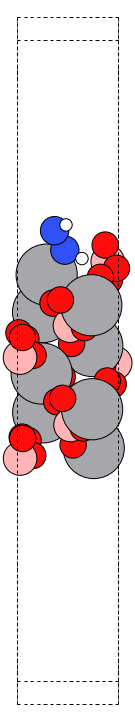
\includegraphics[width=0.15\textwidth, height=85mm]{surface_pathway/N2H2-xside.png}} \\ \hline\ 
H$_{2}$NNH$_{2}$ at top active site&\makecell{  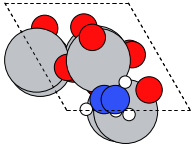
\includegraphics[width=0.30\textwidth, height=38mm]{surface_pathway/H2NNH2-top.png}}&\makecell{  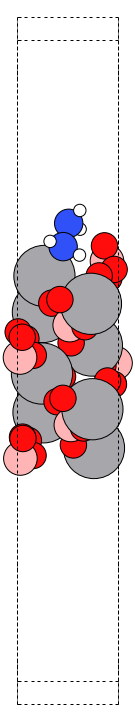
\includegraphics[width=0.15\textwidth, height=85mm]{surface_pathway/H2NNH2-xside.png}} \\ \hline\ 
H$_{2}$NNH at top active site&\makecell{  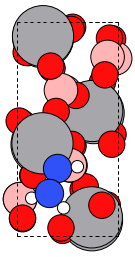
\includegraphics[width=0.30\textwidth, height=38mm]{surface_pathway/H2NNH-top.png}}&\makecell{  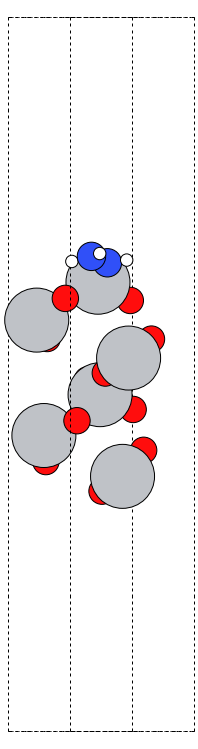
\includegraphics[width=0.15\textwidth, height=85mm]{surface_pathway/H2NNH-xside.png}} \\ \hline\ 
N$_{2}$ at top active site&\makecell{  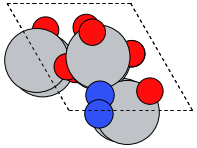
\includegraphics[width=0.30\textwidth, height=38mm]{surface_pathway/N2-top.png}}&\makecell{  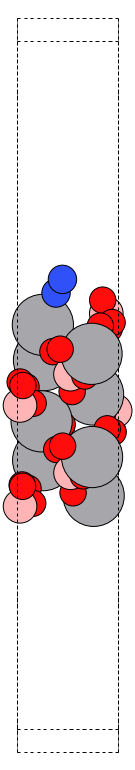
\includegraphics[width=0.15\textwidth, height=85mm]{surface_pathway/N2-xside.png}} \\ \hline \end{longtable}
\end{center}